\documentclass{article}
\usepackage[margin=1in]{geometry}
\usepackage{amsmath,amsthm,amssymb}
\usepackage{bbm,enumerate,mathtools}
\usepackage{tikz,pgfplots}
\usepackage{chessboard}
\usepackage[hidelinks]{hyperref}
\usepackage{multicol} % Problem 35

\newenvironment{question}{\begin{trivlist}\item[\textbf{Question.}]}{\end{trivlist}}
\newenvironment{note}{\begin{trivlist}\item[\textbf{Note.}]}{\end{trivlist}}
\newenvironment{references}{\begin{trivlist}\item[\textbf{References.}]}{\end{trivlist}}
\newenvironment{related}{\begin{trivlist}\item[\textbf{Related.}]\end{trivlist}\begin{enumerate}}{\end{enumerate}}


\begin{document}
\rating{2}{4}
A problem based on a conversation with Alec Jones. Consider a variation on the
``concavity classes'' of polygons as described by OEIS sequence A227910.
Say that two $n$-gons are in the same concavity class if one can be
continuously deformed into the other (or a mirror image of the other) while
(1) remaining an $n$-gon the entire time, and (2) preserving the number of
sides of the convex hull.
\begin{figure}[ht!]
  \centering
  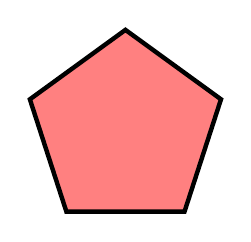
\begin{tikzpicture}[scale=1.5]
    \draw[ultra thick, fill=red!50] (1,0)
      --(0,0)
      --({-cos(72)}, {sin(72)})
      --({-cos(72)+cos(36)}, {sin(72)+sin(36)})
      --({1+cos(72)}, {sin(72)})
      --cycle;
  \end{tikzpicture}\hspace{0.5cm}
  
\begin{tikzpicture}[scale=1.5]
    \draw[ultra thick, fill=orange!50] (0,0)--(1.54/2,1.54/2)--(1.54,0)--(1.54,1.54)--(0,1.54)--cycle;
  \end{tikzpicture}\hspace{0.5cm}
  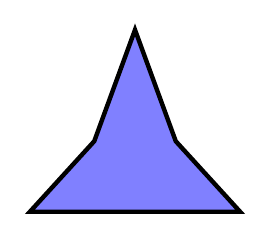
\begin{tikzpicture}[scale=1.5]
    \draw[ultra thick, fill=blue!50] (0,0)
      --({1.78/4 + 0.1}, {1.78*sqrt(3)/4 - 0.1*sqrt(3)})
      --(1.78/2,1.54)
      --({3*1.78/4 - 0.1}, {1.78*sqrt(3)/4 - 0.1*sqrt(3)})
      --(1.78,0)
      --cycle;
  \end{tikzpicture}\hspace{0.5cm}
  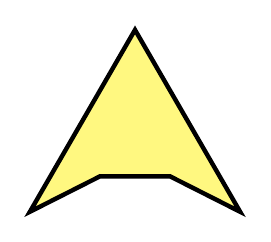
\begin{tikzpicture}[scale=1.5]
    \draw[ultra thick, fill=yellow!50] (0,0)
      --(1.78/2,1.54)
      --(1.78,0)
      --({2*1.78/3}, 0.3)
      --({1.78/3}, 0.3)
      --cycle;
  \end{tikzpicture}\hspace{0.5cm}
  
\begin{tikzpicture}[scale=1.5]
    \draw[ultra thick, fill=green!50] (0,0)
      --(1.78/2,1.54)
      --(1.78,0)
      --({1.78/2}, 0.6)
      --({3*1.78/8}, 0.3)
      --cycle;
  \end{tikzpicture}
  \caption{
    The $a(5) = 5$ concavity classes on the pentagon.
  }
\end{figure}
\begin{question}
  How many convexity classes are there of an arbitrary $n$-gon?
\end{question}

\begin{related}
  \item What is the smallest square lattice that contains at least one
    representative of each concavity class of the $n$-gon for some fixed $n$?
    (That is, the polygons must have integer coordinates.)
  \item (Is this the correct defintion?)
\end{related}
\begin{references}
  \item \url{https://oeis.org/A227910}
\end{references}
\end{document}
